\chapter{Open Questions Examples}

\newquestion
	\paragraph{Question} Derive the continuous-time Fourier transform of AM and PM signals.
	
	\paragraph{Answer} We consider a signal $x(t)$ modulated in amplitude if it can be regarded as a product between a variable amplitude $a(t)$ and a cosine function:
	\[ x(t) = a(t) \cos\big(\Omega_0 t + \phi\big) \]
	It's transform can be computed using the windowing theorem that states that the transform of a product between two signals is the convolution of their transforms, hence 
	\begin{align*}
		X(\Omega) & = A(\Omega) * \left( \frac {e^{j\phi}} 2 \delta\big(\Omega-\Omega_0\big) + \frac {e^{-j\phi}} 2 \delta\big(\Omega+\Omega_0\big) \right) \\
		& = \frac{e^{j\phi}}{2} \intinf A(\theta) \delta\big(\Omega-\theta-\Omega_0\big)\, d\theta + \frac{e^{-j\phi}}{2} \intinf A(\theta) \delta\big(\Omega-\theta+\Omega_0\big)\, d\theta
	\end{align*}
	Knowing the property of the Dirac's delta function $\intinf g(x) \delta(x-x_0) \, dx = g(x_0)$ we can so compute the spectra of the amplitude modulated signal as
	\[ X(\Omega) = \frac{e^{j\theta}}{2} A\big(\Omega-\Omega_0\big) + \frac{e^{-j\theta}}{2} A\big(\Omega+\Omega_0\big)  \]
	This means that the resulting spectrum is a distortion by a complex component $e^{\pm j \theta} / 2$ and shifted by $\pm\Theta_0$ of the spectrum $A(\Omega)$ of the amplitude.
	
	The analysis of signals modulated in phase described in the form $x(t) = A \cos\big(\Omega_0t + \theta(t) \big)$ isn't usually an \textit{easy} problem (analytically manageable \textit{by hand}), but in the simple case
	\[ x(t) = A \cos\big(\Omega_0t + \theta(t)\big) \hspace{2cm} \textrm{with } \theta(t) = k_p \cos(\Omega_pt) \]
	the solution can be obtained. Considering the signal $x(t)$ as the real part of the function
	\[ x(t) = \Re{ A e^{j\Omega_0t} e^{jk_p(\Omega_pt)} } \]	
	
	
\newquestion
	\paragraph{Question} Provide the definition of strict-sense stationary, wide-sense stationary, cyclostationarity and ergodic processes. Explain the relationship between them and why the ergodic properties are particularly useful in practice.
	
	\paragraph{Answer} A strict-sense stationary process is characterized by having a time-invariant mean value and signal power; in particular the probability distribution of the random variables changing with times are always constant, meaning that
	\[ \text{SSS:} \qquad f_{pd,X_n}(x) = f_{pd,X_{n+k}} \qquad \forall k,x \]
	A wide-sense stationary process is a more general definition of strict-sense stationarity, meaning that SSS processes are WSS but not the contrary; this kind of stochastic processes are characterized by a constant mean value $\mu$ for every extracted random variable and the autocorrelation between RVs only depends on the time difference between the extractions
	\[ \text{WSS:} \qquad \mu = \textrm{constant} \quad \text{and} \quad \phi_X(t_1,t_2) = \phi_x \big(t_1-t_2\big)  \]
	Cyclostationarity is a sort of WSS process where the mean and the correlation functions presents a certain periodicity $T_0$, meaning that
	\[ \text{cyclostationarity:} \hspace{2cm} \begin{aligned}
		\mu(t+kT_0) & = \mu(t) \\
		\phi_x(t_1 + kT_0,t_2+kT_0) & = \phi_x(t_1,t_2) 
	\end{aligned} \qquad \forall k\in \mathds Z \]
	Ergodics are all strict-sense stationary processes whose ensemble and time average is equal for every deterministic function $g(\cdot)$, so
	\[ \underbrace{E\big\{ g(X(t)) \big\} = \intinf g(x) f_{pd,X}\, dx }_{\text{ensemble avg.}} = \underbrace{\lim_{T\rightarrow\infty} \frac 1 T \int_{-\frac T2}^{\frac T2} g\Big( x(t,s_i) \Big)\, dx = \big\langle g\big( x(t,s_i) \big) \big\rangle }_{\text{time avg.}} \]
	for every realisation $s_i$ of the random process. Every-time a SSS process is ergodic it means that mean $\mu$, power $P_X$ and autocorrelation $\tau$ of the process can be computed by any realisation of the stochastic process and any \textit{sufficiently big} $T$ as
	\[ \mu = \frac 1 T \int_{-\frac T2}^{\frac T2} x(t,s_i)\, dt \qquad P_X = \frac 1 T \int_{-\frac T2}^{\frac T2} x^2(t,s_i)\, dt \qquad \phi_X(\tau) = \frac 1 T \int_{-\frac T2}^{\frac T2} x(t,s_i)x(t+\tau,s_i)\, dt \]
	
\newquestion
	\paragraph{Question} Prove that the Fourier transform of the convolution of two signals is given by the product of the transforms of the two signals both in the continuous-time and in the discrete-time case.
	
	\paragraph{Solution} Given two discrete time signals $x(n),y(n)$, the convolution between them is given by the formula
	\[ x(n) * y(n) = \infsum k x(n)y(n-k) \]
	By applying on such result the \dtft formulation we obtain
	\begin{align*}
		\four{x(n)*y(n)} & = \infsum n \left( \infsum k x(n)y(n-k) \right) e^{-j\omega n} \\
		& = \infsum n x(n) e^{-j\omega n} \left( \infsum k y(n-k) e^{-j\omega(n-k)} \right) \qquad \textrm{set } u = n-k \\ &  = \infsum n x(n) e^{-j\omega n} \left( \infsum u y(u) e^{-j\omega u } \right) \\
		& = \four{x(n)} \four{y(n)}
	\end{align*}
	
\newquestion
	\paragraph{Question} Compute the mean value, the autocorrelation and the power spectral density (PSD) of the WSS process $y(n)$at the output of a discrete-time LTI system with impulse response $h(n)$, when it is stimulated by a WSS process $x(n)$ with mean $\mu_x$ and autocorrelation $\phi_x(n)$.

	
	\paragraph{Solution} Given the deterministic impulse response $h(n)$ and the WSS input $x(n)$, the output 
	\[ y(n) = x(n) * h(n) \]
	is still a WSS process whose mean can be obtained by computing the first raw statistical moment on the expanded definition of convolution:
	\[ \mu_y = E\{y(n)\} = E\left\{ \infsum k x(n)h(n-k) \right\} = \infsum k h(n-k) E\{ x(n) \} = H\big(e^{j0}\big) \mu_x \]
	where $H(e^{j0})$ is the continuous component of the frequency response of the system. The autocorrelation is still obtained by applying the definition as
	\begin{align*}
		\phi_y\big(y(n),y(n+m)\big) & = E\big\{ y(n) y(n+m)\big\} = E\left\{ \infsum k \infsum r x(n)h(n-k)\,x(n)h(n+m-r) \right\} \\
		& = E\left\{ \infsum k \infsum r x(n-k)h(n)\,x(n+m-r)h(n) \right\} \\
		& = \infsum k \infsum r h(k) h(r) E\big\{ x(n-k)  x(n+m-r) \big\}
	\end{align*}
	Observing that $E\big\{ x(n-k)  x(n+m-r) \big\}$ is equal to the autocorrelation $\phi_x(k+m-r)$, performing the change of variable $l = r - k$ we obtain
	\begin{align*}
		\phi_y\big(y(n),y(n+m)\big) & = \infsum l \phi_x(m-l) \infsum k h(k) h(l+k) = \infsum l \phi_x(m-l) o(l) = \phi_x(m) * o(m)
	\end{align*}
	where $o(l)$ is defined as the convolution $h(l)*h(-l)$. Applying so the DTFT we so obtain the power spectral density of the system as
	\[ \Phi_y\big(e^{j\omega}\big) = H\big(e^{-j\omega}\big) H^*\big(e^{-j\omega}\big) \Phi_x\big(e^{j\omega}\big) = \big|  H\big(e^{j\omega}\big)\big|^2 \Phi_x\big(e^{j\omega}\big) \]
\newquestion
	\paragraph{Question} Show why the convolution operator is associative, commutative and distributive with respect to the addition. As a result, derive the impulse response of the cascade and the parallel of $M$ linear systems.
	
	\paragraph{Answer} Proving the associative property means ensuring that $x(n)*y(n)*z(n) = \big(x(n)*y(n)\big)*z(n) = x(n) * \big( y(n) * z(n) \big)$; such equality is simply verified using the Fourier transform: known in fact that $\four{v(n)* w(n)} = V(e^{j\omega}) W(e^{j\omega})$ then it means that
	\[ X\big(e^{j\omega}\big) Y\big(e^{j\omega}\big) Z\big(e^{j\omega}\big) = \Big(X\big(e^{j\omega}\big) Y\big(e^{j\omega}\big)\Big) Z\big(e^{j\omega}\big) = X \big(e^{j\omega}\big) \Big(Y\big(e^{j\omega}\big)Z\big(e^{j\omega}\big)\Big) \]
	Being the product an associative operation, this means that the all the relationships in the frequency domain are verified and so the the convolution is proven to be associative. The commutative property is still proven considering the commutativity of the multiplication applied in the frequency domain, in fact
	\[ X\big(e^{j\omega}\big) Y \big(e^{j\omega}\big) = Y\big(e^{j\omega}\big) X\big(e^{j\omega}\big) \qquad \Rightarrow \qquad x(n)*y(n) = y(n)*x(n) \]
	Knowing that the Fourier transform is a linear operator, meaning that for every $a,b\in \mathds R$ we have that $\four{a\, x(n) + b\,y(n)} = aX(e^{j\omega}) + bY(e^{j\omega})$, then we can also prove the distributive property of the convolution:
	\[ \big(x(n) + y(n)\big)* z(n) = x(n)*z(n) + y(n)*z(n) \]\[ \xrightarrow{\F} \qquad \Big( X\big(e^{j\omega}\big) + Y\big(e^{j\omega}\big)\Big) Z\big(e^{j\omega}\big) = X\big(e^{j\omega}\big)Z\big(e^{j\omega}\big) + Y\big(e^{j\omega}\big)Z\big(e^{j\omega}\big)  \]
	Being the multiplication a distributive operation, the distributivity of the convolution is so proven.
	
	The output $y(n)$ of a system made by $M$ linear systems in parallel connection is equal to the sum of all the output for the independent stages, meaning that
	\[ y(n) = \sum_{i=0}^{M-1} y_i(n) \]
	Knowing that the output of each stage can be computed by the convolution between it's input $x_i(n)$ and the impulse response $h_i(n)$ as $y_i(n) = x_i(n)*h_i(n)$, having all inputs $x_i(n)$ equal to one input $x$ then we have 
	\[ y(n) = \sum_{i=0}^{M-1} y_i(n) = \sum_{i=0}^{M-1} x_i(n)*h_i(n) = x(n) * \sum_{i=0}^{M-1} h_i(n) = x(n) * \Big(h_0(n) + \dots + h_{M-1}(n)\Big)\]
	
\newquestion
	\paragraph{Question} Spectral estimation of deterministic signals: methodology, and main uncertainty sources
	
	\paragraph{Answer} To estimate deterministic signals we have to rely on discrete-time system, meaning that the original continuous-time function $x_c(t)$ must be sampled with a period $T_s$ that might lead to the generation of spectral replicas: the sampled spectrum $X(e^{j\omega})$ is in fact
	\[ X \big(e^{j\omega}\big) = \frac 1{T_s} \infsum k X_c\left( \frac{\omega}{T_s} + \frac{2\pi k}{T_s} \right) \]
	After this discretization in the time domain, to numerically process the data we cannot use the whole samples collected but only a finite subset. Mathematically this means multiplying the samples signal $x(n)$ with a proper window function $w(n)$ (that for the simplest case is the rectangular one); the signal that can so be analysed is $v(n) = x(n)w(n)$ whose spectrum is a distorted version of $X(e^{j\omega})$ due to the windowing theorem, in fact
	\[ V\big(e^{j\omega}\big) = X\big(e^{j\omega}\big)*W\big(e^{j\omega}\big) \]
	This distortion leads to the spectral leakage phenomena on which the energy of the signal is dispersed all over the frequency axis; the windowed spectrum $V(e^{j\omega})$ is in fact distorted by the convolution operation. Window function usually presents a \textit{Dirichlet-Kernel-like} shape with a main-lobe centred at the pulsating frequency and side-lobes leaking the energy of the signal. Different window might determine, for the same length $L$, narrower main-lobe width (improving so the theoretical resolution of the estimation) with the draw-back of a higher side-to-main-lobe ratio (increasing the problem of spectral infiltration).\\
	Lastly the estimation is performed not on the \dtft (that continuous in the frequency), but on it's sampled version (the DFT); depending so on the number of samples used to estimate the spectrum, we might read only the spectrum of interest (case of coherent sampling for pure sinusoidal sequence) or we can read only effects of spectral leakage and infiltration (non-coherent sampling).
	
\newquestion
	\paragraph{Question} Provide a definition of spectral resolution and explain how it can be determined. Describe the trade-off 	between time vs. spectral resolution in the case of non-stationary signals and explain the meaning of "uncertainty principle".
	
	\paragraph{Answer} Considering the case of a stationary continuous-time signal determined as the sum of two sinusoidal function $x_c(t) = A_1\cos(\Omega_1t + \phi_1) + A_2 \cos(\Omega_2 t + \phi_2)$, the expected transform consists in 4 Dirac pulses centred at frequencies $\pm \Omega_1,\pm \Omega_2$. Assuming that by discretizing the sequence $x(n)$ no aliasing  occurs, the theoretical DTFT still presents pulses at frequencies $\pm \omega_1 = \Omega_1 = \Omega_1 T_s$ and $\pm \omega_2 = \Omega_2 T_s$. \\
	After the windowing of the discretized signal $x(n)$, the analysed sequence $v(n) = x(n) w(n)$ presents a spectral distortion due to the windowing theorem as
	\[ V\big(e^{j\omega}\big) = X\big(e^{j\omega}\big) * W\big(e^{j\omega}\big)  \]
	This window determines a spectral leakage that spreads the energy that's theoretically held only by the Kronecker pulse on all the frequency axis; the window's transforms presents a \textit{Dirichlet-Kernel-shaped} function characterized by a main-lobe with a width $\Delta$. If it happens that the frequencies $\omega_1,\omega_2$ are closer then the distance $\Delta/2$ it means that the main-lobes of the windowed signal majorly overlaps, resulting in a constructive spectra that \textit{erase} the initial detached main-lobes centred at $\omega_1,\omega_2$ but generates a unique main-lobe. This means that given the main-lobe width $\Delta$ (function of the length $L$ of the window), the resolution in the frequency domain that we obtain is $\Delta/2$.
	
	Considering so non-stationary signals, in order to keep track of the changes in the property of the signal it's necessary to sample short time ranges (and so analyse narrower time windows but with more frequency): this inevitably leads a to a fewer samples to be processed (in the assumption that the sampling frequency is known and fixed) that results in a broader main-lobe width negatively impacting the frequency resolution. Contrary bigger windows in time allow to collect more samples (better frequency resolution) but doesn't allow to track changes in time of the property of the signal. In general given a window in time of width $\Delta t$, the maximum frequency resolution $\delta_f$ follows the inequality
	\[ \delta_f \, \Delta t > 1  \]
	
\newquestion
	\paragraph{Question} Show the effect of down-sampling/decimation on a generic signal both graphically and mathematically.	What is the main risk of down-sampling? How can we solve the problem?
	
	\paragraph{Answer} The down-sampling with a decimation factor $M$ is used to reduce the data to process (when for example processors cannot perform real-time operation with such quantity of data) by simply analysing 1 sample each $M$ values collected. Mathematically given the initial sequence $x(n)$, the decimated one is expressed as
	\[ x_d(n) = x(nM) \qquad \textrm{with } M \in \mathds N \]
	The main risk of down-sampling is the aliasing problem: as for the continuous-to-discrete time conversion only frequencies $\Omega \leq \pi / T_s$ where able to be sampled with no frequency aliasing, similarly decimating the sequence means increasing the sampling time and so the maximum allowed analog frequency is
	\[ \Omega \leq \frac{\pi}{MT_s} \]
	By a spectral point of view the continuous-time spectra $X_c(\Omega)$ is so sampled with a period $T_s' = MT_s$ determining 
	\[ X_d\big(e^{j\omega}\big) = \frac 1{T_s'} \infsum k X_c\left( \frac{\omega}{T_s'} + \frac{2\pi k}{T_s'} \right) = \frac 1{MT_s} \infsum k X_c\left( \frac{\omega}{MT_s} + \frac{2\pi k}{MT_s} \right)\]
	Graphically the relation between original discretized sequence spectrum and decimated one is shown as
	\begin{center}
		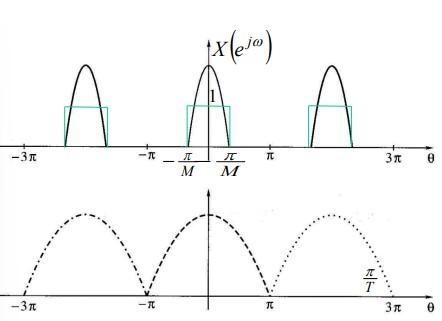
\includegraphics[width=6cm]{downsampling}
	\end{center}

	To solve the possible occurrence of aliasing a low pass filter with cut-off frequency $\omega_c = \pi/M$ and unitary gain must be inserted before the the decimator block.
	
\newquestion
	\paragraph{Question} Periodograms and modified periodograms: definitions and statistical properties in terms of bias and	variance. Explain why and under which assumptions the average periodogram can improve spectral	estimation.
	
	\paragraph{Answer} Periodograms are used to estimate the power spectral density (and so the DTFT of the autocorrelation of a windowed signal $v(n) = x(n)w(n)$ with length $L$) directly in the frequency domain. The formulation of the periodogram and the modified periodogram is respectively
	\[ \Phi_V(\cdot) = \frac{|V(\cdot)|^2}{ L } \hspace{2cm} \Phi_V(\cdot) = \frac{|V(\cdot)|^2}{\sum_{i=0}^{L-1} w(i)} \]
	In particular we can see that the \textit{basic} periodogram is the modified one assuming a rectangular window. By computing the expected value for any generic input we determine that
	\[ E\{\Phi_V\} = \frac 1 L \phi_x(e^{j\omega}) * |W(e^{j\omega})|^2 \]
	and so the periodogram is asymptotically unbiased, meaning that for $L\rightarrow \infty$ (bigger windows) the estimated value tends to coincide with the \textit{real} one. Regarding it's consistency it's necessary to compute the variance
	\[ \var{\Phi_V} = E\{ \Phi_V^2 \} \propto \Phi_X^2(e^{j\omega}) \]
	and so we can see that, even with $L\rightarrow \infty$, the periodogram is still an inconsistent estimator.
	
\newquestion
	\paragraph{Question} FIR filter design based on the windowing method: general idea and motivation, role and features of different windows and filter design steps. Briefly explain pros and cons of the algorithmic FIR filter design techniques compared to the classic windowing method.
	
	\paragraph{Answer} Finite impulse response filter are usually preferable due to their (generalized) linear phase behaviour. The main idea behind the design of a FIR filter starts firstly from determining the ideal impulse response by simply inverting the chosen window; this process generates an non-causal infinite impulse response (that wasn't the goal of the filter and is also practically not feasible) that however can be truncated up to a number of samples $M$ and shifted by $M/2$ samples. \\
	By computing the new transfer function in the frequency domain considering the windowing theorem is possible to observe that this process generates ripples with fixed amplitude (independent on the length $M$ of the filter) and a transition bandwidth function of $M$. In general the design steps to follow to design such kind of filter are:
	\begin{itemize}
		\item compute the ideal impulse response $h_{id}(n)$ of the chosen filter;
		\item given the specification of the maximum amplitude $\delta$ chose from the tabled window functions the one that has a maximum ripple amplitude $\varepsilon < \delta_{dB} = 20\log_{10}\delta$; known the transition bandwidth $\Delta \omega$ from the specification determine the value of $M$ that presents a main-lobe width $\Delta_w$ less than such value;
		
		\item compute the impulse response as $h(n) = h_{id} \left( n - \frac M2\right) w(n)$ using the chosen window function;
		
		\item check the compliance of the so generated transfer function with the initial specification; if necessary iterate this process.
	\end{itemize}
	
\newquestion
	\paragraph{Question} Describe and explain in detail the design steps of a low-pass IIR filter.
	
	\paragraph{Answer} The design of a digital low-pass filter (with unitary gain) has to start by firstly determining it's specification, so:
	\begin{itemize}
		\item the maximum deviation $\delta_1$ in the pass-band region; this means that allowed value of the output of the filter must be bound in the range $[1-\delta_1,1]$;
		\item the maximum deviation $\delta_2$ in the stop-band region; the range of the allowed values in this region is so $[0,\delta_2]$;
		\item the maximum pass-band frequency $\omega_p$;
		\item the minimum stop-band frequency $\omega_s$.
	\end{itemize}
	With this value determined (if necessary transform decibels value into the related \textit{linear} scale) the design of the filter follows this step:
	\begin{enumerate}
		\item firstly we want reconduct the design of a discrete-time filter to a continuous-time on, the low-pass prototype (where design equation/parameters are well known). Deduced by the bilinear transform we can compute the analog frequencies $\Omega_p,\Omega_s$ respectively of the pass/stop-band as
		\[ \Omega_p = \frac 2 T \tan\left( \frac{\omega_p}2 \right) \hspace{2cm} \Omega_s = \frac 2 T \tan\left( \frac{\omega_s}2 \right) \]
		In this case the discretization time $T$ value is arbitrary and can be chosen at will (considering that the same value must be used later on in step 3);
		
		\item in this stage we have to design the low-pass prototype in the analog domain and the related transfer function. Considering as example the Butterworth filter characterized by a magnitude response
		\[ |H_c(\Omega)|^2 = \frac{1}{1-\left(\frac{\Omega}{\Omega_c}\right)^{2N}} \]
		The minimum order $N$ of the filter and it's cut-off frequency $\Omega_c$ are determined with the equation
		\[ N = \left\lceil  \frac{ \ln \left( \dfrac{ \frac{1}{\delta_2^2} -1 }{\frac 1{(1-\delta_1)^2} - 1} \right)  }{ 2\ln \left(\dfrac{\Omega_s}{\Omega_p}\right)}  \right\rceil \hspace{1.5cm} \Omega_c = \frac{\Omega_s}{\sqrt[2N]{ \frac{1} {\delta_2^2}-1}}   \]
		The continuous transfer function $H_c(s)$ in the Laplace domain is so characterized by the equation
		\[ H_c(s) = \frac{ \Omega_c^N }{\prod_{k=0}^{N-1} \big(s-s_k\big)} \]
		where the $t$-th pole is obtained (for the Butterworth case) as
		\[ s_k = \Omega_c\Big( \cos\phi_k + j \sin\phi_k \Big)  \qquad \textrm{with } \phi_k = \frac \pi 2 + \big(2k+1\big) \frac{\pi}{2N} \quad \forall k=0,\dots, N-1 \]
		
		\item knowing the transfer function of the continuous-time prototype, the discrete filter is obtained by the bilinear transform on such computed transfer function, so by computing
		\[ H(z) = H_c(s) \Big|_{ s= \frac 2 T \frac{1-z^{-1}}{1+z^{-1}} } \]
		where the time $T$ is the value chosen at step 1; after numerical manipulation is possible to compute a transfer function that's a rational polynomial can so be represented by graphs.
	\end{enumerate}

\newquestion
	\paragraph{Question} Describe and explain the structure of an ideal C/D converter and a real Analog-to-Digital Converter (ADC). Sketch the schematic and explain the principle of operation of a flash ADC circuit.

	
	\paragraph{Answer} The block that perform the conversion of a continuous-time continuous-valued function $x_c(t)$ into  a discrete-time discrete-valued signal $x(n)$ is mainly perform by the following blocks:
	\begin{itemize}
		\item the \textit{sample \& hold amplifier} whose goal is to discretize the time axis with a sampling period $T_s$. Such discretization might lead to aliasing in the frequency domain so usually an analog anti-aliasing low-pass filter should be put in front of the sample \& hold. A \textit{zero order hold} system is necessary to rapidly \textit{track} the continuous input signal $x_c(t)$ and then maintain for the rest of the period the output constant to the read value generating the sequence $x(n)$;
		
		\item consequently the ADC block performs the proper conversion by quantizing the value $x(t)$ and decoding it into a binary value in order to allow digital processing. Usually this operation are performed together (the same circuit is used for both quantization of the values and binary codification).
	\end{itemize}
	
	\textbf{MANCA DA SPIEGARE IL FLASH ADC}

\newquestion
	\paragraph{Question} Describe and explain the structure of an ideal D/C converter and a real Digital-to-Analog Converter (DAC). Sketch the schematic and briefly explain the principle of operation of an R-2R DAC.
	
	\paragraph{Answer} To perform a real digital to analog conversion the following block should be involved:
	\begin{itemize}
		\item a decoder used to decode binary digit into the corresponding analog value;
		
		\item a sample \& hold operation (usually implemented together with the decoder) that allow to re-introduce the concept of time that was lost in the discretization: the decoded signal is maintained constant at the output of the zero order hold for a period $T_s$ equivalent to the one used in the sampling process;
		
		\item a low-pass reconstruction filter that attenuates the effects of the window distortion on the signal.
	\end{itemize}
	\textbf{MANCA IL R-2R LADDER}
	
\newquestion
	\paragraph{Question} Provide the definition of system linearity, causality, time-invariance and BIBO stability. Also, prove why	in an LTI discrete-time system asymptotic stability is guaranteed if and only if all poles of the transfer function lie within the unit circle.
	
	\paragraph{Answer} A system characterized by a transfer function $T\{\cdot\}$ is defined
	\begin{itemize}
		\item linear if the output of any linear combination maps to the linear combination of the single outputs, meaning that
		\[ T \{ a\, x(\cdot) +b\, y(\cdot)\} = a\, T\{x(\cdot)\} + b \, T\{ y(\cdot)\} \qquad \forall a,b\in \mathds R \ x(\cdot),y(\cdot) \textrm{ function} \]
		This means that a system can be described by matrix calculus;
		
		\item time-invariant if the transfer function $T\{\cdot\}$ doesn't change with time;  intuitively it means that if the initial status of the system is set to a known value, the output behaviour of the system subjected to a causal signal $x(\cdot)$ is independent from the time $t$ on which the input occurs;
		
		\item causal if the system's output strictly depends on past and/or current inputs, but not the future's one;
		
		\item BIBO stable if for any bounded-input $x(\cdot) < M$ the output is also bounded, so $\exists N$ such that $ |y(\cdot)| = |T\{x(\cdot)\}| < N$.		
	\end{itemize}

	For discrete-time causal LTI system characterized by a transfer function $H(z)$ that's a rational polynomial
	\[ H(z) = \frac{N(z)}{D(z)} = Q(z) + \frac{R(z)}{D(z)} \]
	such ratio can be split into a simple polynomial that inversed determine a finite impulse response; the second remaining rational term $R(z)/Q(z)$ can be further decomposed using the partial fraction expansion. In the simplified case on which all the poles are real and with unitary molteplicity such decomposition is in the form
	\[ \frac{R(z)}{D(z)} = \frac{A_1}{1-p_1 z^{-1}} +  \frac{A_2}{1-p_2 z^{-1}} + \dots \]
	The computing the inverse Z transform we have that
	\[ \mathcal Z ^{-1} \left\{ \frac 1 {1-az^{-1}} \right\} = a^nu(n) \]
	where the region of convergence in order to obtain such value was $|a| < 1$; this means that if all the poles of the transfer function lie within the unit circle then the transform belongs to the region of convergence; if $|a|\leq 1$ the causal exponential $a^nu(n)$ asymptotically tends to $0$ and so this proves that the system is asymptotically stable.
	
\newquestion
	\paragraph{Question} Describe the decimation-in-time FFT algorithm over $N = 2^\nu$
	samples and explain why algorithm complexity is $\mathcal O(N \log_2 N)$.

	
	\paragraph{Answer} To understand the decimation in time algorithm we firstly need to state the DFT definition that's
	\[ X(k) = \sum_{n=0}^{N-1} x(n) e^{j\frac{2\pi}{N}kn} = \sum_{n=0}^{N-1} x(n) W_N^{kn} \hspace{2cm} \forall k=0,\dots,N-1 \]
	where $W_N = e^{j\frac{2\pi}{N}}$ is the \textit{twiddle factor}. The idea of the decimation in time algorithm is to divide the original sequence $x(n)$ into an even $x_e$ and an odd $x_o$ one, and so
	\[ x_e(r) = x(2r) \qquad x_o(r) = x(2r+1) \hspace{2cm} r =0,\dots, N^{\nu - 1} - 1 \]
	\begin{align*}
		\Rightarrow \quad X(k) & = \sum_{n=0}^{N-1} x(n) W_N^{kn} = \sum_{r=0}^{\frac N2-1} x_e(r) W_{N}^{2rk} + W_N^{k} \sum_{r=0}^{\frac N2-1} x_o(r) W_{N}^{2rk}		
		\\ & = \sum_{r=0}^{\frac N2-1} x_e(r) W_{N/2}^{rk} + W_N^{k} \sum_{r=0}^{\frac N2-1} x_o(r) W_{N/2}^{rk} \\		
		& = X_e(n) + W_N^kX_o(k)
	\end{align*}
	where the result has been obtained considering that for the twiddle factor $W_{N}^2 = W_{N/2}$. Computationally the idea is to continue splitting the original sequence $x(n)$ into subsequences of even/odd position (the assumption of having $N=2^\nu$ ensures that this operation is always possible) until we have a sequences $x(0),x(1)$ made just by two elements whose spectral components can be computed as
	\[ X(0) = x(0)+x(1) \hspace{2cm} X(1) = x(0) - x(1) \]
	With all the pairs subsequences computed the transforms are re-combined using the same butterfly graph with different weight of the edges depending on the twiddle factors.
	
	From a computational standpoint, the pure definition of the DFT is $\mathcal O (N^2)$: for every $k$-th sample (with $k=0,\dots,N-1$) a summation of $N$ terms has to be performed. Applying the decimation in time FFT algorithm the computational cost seems to be equal, however the computation of the single odd + even spectrum is numerically lighter than the full expression; to continuos iterative formulation allows so to reach the asymptotic complexity $\mathcal O(N\log_2N)$ typical of dichotomous algorithms.

\newquestion
	\paragraph{Question} Explain the relationship between the DIT FFT, the DIF FFT algorithms and the respective inverse Fast Fourier Transforms. Compute and compare the number of real-valued operations of a classic FFT with respect to a standard DFT when $N = 1024$ points are considered.
	
	\paragraph{Answer}	\textbf{DA FARE}
	
\newquestion
	\paragraph{Question} Show why an FIR system of type I exhibits a linear phase response. Where are the zeros and the poles	of its transfer function located in the $z$ complex plane?
	
	\paragraph{Answer} A FIR of type I is characterized by a symmetric impulse response in the form
	\[ h(n) = h(M-n) \qquad \textrm{with $M$ even} \]
	Writing such impulse response as
	\[ h(n) = \sum_{k=0}^{M-1} b_k \delta(n-k) 	\qquad \textrm{with } b_k = b_{M-k} \]
	to prove it's linear phase response is necessary to compute it's \dtft that, considering the particular symmetry of the impulse response, can be regarded as
	\begin{align*}
		H\big(e^{j\omega}\big) & = b_{M/2} e^{-j\omega \frac M2} + \sum_{n=0}^{\frac M2-1} b_n \left( e^{-j\omega n} + e^{-j\omega(M-N)} \right) \\
		& = e^{-j\omega \frac M 2} \left( b_{M/2} + \sum_{n=0}^{\frac M2-1} 2 b_n \left( \frac{e^{j\omega\left( \frac M 2 - n \right)} +e^{-j\omega\left( \frac M 2 - n \right)} }{2} \right) \right) \\
		& = e^{-j\omega \frac M 2} \left( b_{M/2} + \sum_{m=0}^{\frac M2-1} 2 b_m \left( \frac{e^{j\omega m } +e^{-j\omega m} }{2} \right) \right) \\
		& = e^{-j\omega \frac M 2} \sum_{m=0}^{M/2} c_m \cos(\omega m) = e^{-j\omega \frac M2} A_e(\omega)
	\end{align*}
	Considering that $A_e(\omega)$ is a real evaluated signal with an even symmetry, then the overall phase response is linear depending on the contribution of $e^{-j\omega \frac M2}$.
	
	
	
\newquestion
	\paragraph{Question} Explain the effect of up-sampling and interpolation both graphically and analytically. What is the main problem of ideal interpolators and how can we mitigate it?
	
	\paragraph{Answer} The upsampling is the operation that virtually increases the number of samples in the sequence; given an interpolation factor $L$ such operation performs a zero padding of $L-1$ zeros after each sample, so given the initial sequence $x(n)$, the expanded one is defined as
	\[ x_e(n) = \begin{cases}
		x(n/L) \qquad & n = 0,\pm L, \pm 2L,\dots \\ 0 & \textrm{otherwise}
	\end{cases} \]
	This operation inevitably changes the spectrum of the original signal that now seems distorted due to the time shift property:
	\[  X_e\big(e^{j\omega}\big) = \infsum n x_e(n) e^{-j\omega n} = \infsum k x(k) e^{-j\omega k L} = X\big(e^{j\omega L}\big) = X\big(e^{j\omega'}\big) \]
	Applying the definition of the spectrum $X(e^{j\omega})$ determined from the continuous one $X(\Omega)$ and keeping in mind that $\omega' = \omega L$ (hence $T_s' = T_s/L$) we obtain the spectra
	\[ X_e\big(e^{j\omega}\big) = X\big( e^{j\omega'}\big) = \frac 1 {T_s} \infsum k X_c\left( \frac{\omega'}{T_s} - \frac{2\pi k}{T_s} \right) = \frac 1{LT_s'} \infsum k X_c \left( \frac \omega {T_s'} - \frac{2\pi k}{LT_s'} \right) \]
	Graphically all the spectral replicas are compressed by a multiplicative factor $1/L$ in magnitude and are whole axis is \textit{shrinked} by a factor $1/L$: if before we had 2 replicas in a range $[0,2\pi]$, now they became $L$. In order to recover this two problems it's necessary to use a low pass interpolator filter with a gain $L$ in the pass-band (in order to restore the original magnitude) and a discretized cut-off frequency $\omega_c = \pi /L$.
	
\newquestion
	\paragraph{Question} Considering an ideal RC analog low-pass filter, show how this system can be discretized and described by a constant coefficient linear difference equation.

	
	\paragraph{Answer} To determine the constant linear difference equation of the RC circuit firstly is important to express the differential equation that physically describes the problem:
	\[ x(t) = Ri(t) + y(t) = RC \dot y(t) + y(t) \]
	where $x(t)$ is the input and $y(t)$ is the output voltage of the system. Considering so that the derivative $\dot y(n)$ can be numerically approximated for discrete-time sequences
	\[ \dot y(n) \approx \frac{y(n)-y(n-1)}{T} \]
	where $T$ is the time step, then the original differential equation can be approximated as
	\[ x(n) = RC \frac{y(n)-y(n-1)}{T} + y(n) \]
	To constant coefficient liner difference equation is so obtained by solving the discretized model for the current output $y(n)$ as function of the previous outputs and the input history:
	\begin{align*}
		y(n) \left( \frac T{RC} + 1\right) & = \frac T{RC} x(n) + y(n-1) \\
		y(n) & = \frac{\frac T{RC} x(n) + y(n-1) }{\frac T{RC} + 1} = \frac{T }{RC+T} x(n) + \frac{RC}{RC+T}y(n-1) \\ 
		& = a \, y(n-1) + b\, x(n)
	\end{align*}
	where 
	\[ a = \frac{RC}{RC+T} = \frac{1}{1 + \frac{T}{RC}} \hspace{2cm} b = \frac{T}{RC+T} = 1-a \]
	
\newquestion
	\paragraph{Question} Provide the definition of deterministic autocorrelation in the continuous-time and discrete-time domain and compute the corresponding Fourier transforms.
	
	\paragraph{Answer} Given a signal $x(\cdot)$ it's deterministic autocorrelation $\phi_x(\tau)$ tends to measure \textit{how much correlation} there is between a signal and itself shifted in time by a value $\tau$ (1 high correlation, 0 no correlation), in particular the definition for both continuous and discrete-time case are
	\[ \phi_x(\tau) = \intinf x(t)x^*(t+\tau)\, dt =x(t)*x^*(-t) \hspace{2cm} \phi_x(k) = \infsum n x(n) x^*(n+k) \]
	Considering that the autocorrelation can be regarded as the expectation $\phi_x = E\{x(t_1)x^*(t_2)\}$ then it means that it's autocorrelation is a constant function
	\[ \phi_x(\tau) = E\{ x(t) x^*(t+\tau) \} = \intinf x(t)x^*(t+\tau) \, dt\]
	
	
	Usually deterministic signals presents a finite energy and in most cases are also infinitely summable, hence the Fourier transform can be applied on the signal as
	\[ \Phi_x(\Omega) = \intinf \phi_x(\tau) e^{-j\Omega \tau}\, d\tau \hspace{2cm} \Phi_x \big(e^{j\omega}\big) = \int_{-\pi}^\pi \phi_x(\tau) e^{-j\Omega \tau}\, d\tau \]
	
	\textbf{DA RIVEDERE}

\newquestion
	\paragraph{Question} What properties should the impulse response have to make an LTI system BIBO stable and causal? Justify your answer analytically
	
	\paragraph{Answer} Firstly, in order to have causality, we have to ensure that the impulse response is non-zero only for $t,n\geq 0$: by computing in fact the convolution $x(\cdot)*h(\cdot)$ the output $y(\cdot)$ strictly depends on the current/past inputs/states if and only if the impulse response matches the previously state requirement.\\
	For the BIBO stability is instead required that every value $h(\cdot)$ of the impulse response is finite: the linear combination of finite sums can still be bounded by a value (even if it's \textit{very high}).
	
\newquestion
	\paragraph{Question} Prove and explain why a filter with a linear phase response does not introduce any phase distortion. Can we design IIR filter without phase distortion? Why?

	
	\paragraph{Answer} \textbf{DA FARE}
	
\newquestion
	\paragraph{Question} Provide the definition of random power and energy signals. Prove why the SSS and WSS random processes can just be power signals.
	 
	\paragraph{Answer} A function $x(\cdot)$ is defined as energy signal if it's energy $E$ (regarded as the signal squared integrated in the whole domain) is finite; this means computing (for both the continuous and discrete-time case) the values
	\[ E = \intinf |x(t)|^2\, dt < \infty \hspace{2cm} E = \infsum k |x(k)|^2 < \infty \]
	Real signals (generally) has to present  a finite energy, but considering that they are usually modelled as stochastic processes where each extracted random variable is characterized by a PDF (usually known up to the second statistical moment, so mean and variance), their integration over time results in an infinite energy (and so the realization of stochastic process cannot be regarded as energy signals); however this representation of signals present a finite power $P$ defined (for the continuous-time case) as
	\[ P = \lim_{T\rightarrow\infty} \frac 1 T\int_{-\frac T2}^{\frac T2} |x(t)|^2\, dt \]
	
	\textbf{DA FINIRE}
	
\newquestion
	\paragraph{Question} Explain and prove why the discretization of an LTI system based on the bilinear transform preserves system stability and how the analog frequency $\Omega$ is mapped/transformed into the normalized one $\omega$.

	
	\paragraph{Answer} The bilinear transform is obtained considering the expansion of the derivative $y(\cdot) = \dot x(\cdot)$ in both the Laplace (continuous-time function) and Z domain (discrete-time function); considering in fact the continuous-time case we obtain that
	\[ \frac{Y(s)}{X(s)} = s \]
	while for discrete-time signal the differentiation can be approximated using the trapezoidal rule as
	\[ \frac{x(n) - x(n-1)}{T} = \frac{y(n)+y(n-1)}{2} \qquad \xrightarrow{\mathcal Z} \qquad \frac{X(z) - z^{-1}X(z)}T = \frac{Y(z) + z^{-1}Y(z)}{2}  \]
	\[ \frac{Y(z)}{X(z)} = \frac{2}{T} \frac{1-z^{-1}}{1+z^{-1}} \]
	Equating the transfer function for the continuous and discretized-time case we obtain the bilinear transform
	\[ s = \frac{2}{T} \frac{1-z^{-1}}{1+z^{-1}} \]
	Knowing that the CTFT is the evaluation of the Laplace transform for $s=j\Omega$ and the DTFT is the evaluation of the $z$ variable in $e^{j\omega}$, we can solve the bilinear transform in order to retrieve $\Omega$ as function of $\omega$ and vice-versa:
	\[ j\Omega = \frac 2 T \frac{1-e^{-j\omega}}{1+e^{-j\omega}} \qquad \Rightarrow \qquad \Omega = \frac 2 T \tan\left(\frac \omega 2\right) \quad \leftrightarrow \quad \omega = 2 \arctan\left( \frac{T\Omega}{2} \right)\]
	Knowing that the spectra of a continuous-time system is defined in the set $[-\infty,\infty]$ we can see that the bilinear transform doesn't generate any spectral replica because the spectrum is mapped in the domain of the transform for discrete-time signals:
	\[ \Omega: [-\infty,\infty] \quad \mapsto \quad \omega:[-\pi,\pi] \]
	
	To check how such transformation preserves stability is more useful to revert the bilinear transform in order to express $z$ as function of $s$ and so
	\begin{align*}
		Ts \left( 1 + \frac 1 z\right) & = 2 \left(1 - \frac 1 z\right) \\
		Ts \big(z+1\big) & = 2\big(z-1\big) \\
		\big(Ts-2\big) z & = -Ts - 2 \\
		z &= - \frac{Ts + 2}{Ts-2} = \frac{1 +\frac T2 s}{1 - \frac T2 s}
	\end{align*}
	We can so see that whenever $\Re{s} > 0 $ (and so the poles for continuous-time systems are unstable) the module of the numerator is bigger then the one of the denominator, hence $|z|>1$ resulting in unstable poles for the discrete-time systems. When instead $\Re{s}<0$ we can similarly prove that the poles are transformed in the stable region $|z|<1$ for the Z transform. In the particular case where $\Re{s} = 0$ we have that numerators and denominator are complex conjugates and their modules are equals, hence $|z| = 1$.
	
\newquestion
	\paragraph{Question} Prove that wide-sense stationary processes can only be power signals.
	
	\paragraph{Answer} The energy $\mathcal E$ of a stochastic process $X(t)$ is determined by the second order raw statistical moment $E\{X^2(t)\}$ hence
	\[ \mathcal E = \intinf E\{ X^2(t) \} \,dt = \intinf E\{x^2(t)\}\, dt = \intinf \phi_X(t)\, dt \]
	In case of wide-sense stationary random processes the autocorrelation function $\phi_X(t)$ is constant to $\phi_X(0)$, hence the energy diverges to infinity:
	\[ \mathcal E = \intinf \phi_X(0)\, dt = \infty  \]
	However if we consider the power $\mathcal P$ of the signal we have that in the case of wide-sense stationary stochastic processes
	\[ \mathcal P = \lim_{T\rightarrow \infty} \frac 1{2T} \int_{-T}^T E\{x^2(t)\} \, dt = \lim_{T\rightarrow \infty} \frac 1{2T} \int_{-T}^T \phi_X(0) = \lim_{T\rightarrow \infty}  \cancel{\frac 1 {2T} 2T}\phi_X(0) = \phi_X(0) \]
	
	
	
	
	
	
	
	
	
	
	
	
	
	
	